% !TeX program = xelatex
% !TeX encoding = UTF-8
% !TeX spellcheck = en_US
% !BIB program = biber
%% 
%% The above lines help editors like TeXstudio to automatically choose the right tools
%% to compile your LaTeX source file. If your tool does not support these magic comments,
%% you will need to make appropriate manual choices.
%% 
%% You can safely use "pdflatex" instead of "xelatex" if you prefer the pdfLaTeX toolchain.
%% However, pdfLaTeX will not be able to deliver the professional font experience that you
%% will get with XeLaTeX. You can also safely use "lualatex" instead of "xelatex" while
%% preserving the professional font experience if you prefer the LuaLaTeX toolchain.
%% 
%% _Important_: These magic comments should be on the first lines of your source file.
%% 
%%%%%%%%%%%%%%%%%%%%%%%%%%%%%%%%%%%%%%%%%%%%%%%%%%%%%%%%%%%%%%%%%%%%%%%%%%%%%%%%

%%%%%%%%%%%%%%%%%%%%%%%%%%%%%%%%%%%%%%%%%%%%%%%%%%%%%%%%%%%%%%%%%%%%%%%%%%%%%%%%
%% 
%%            JJJJ   K                         K   UUUU         UUUU  
%%            JJJJ   KKKK                   KKKK   UUUU         UUUU  
%%            JJJJ   KKKKKK               KKKKKK   UUUU         UUUU  
%%            JJJJ      KKKKKK         KKKKKK      UUUU         UUUU  
%%            JJJJ         KKKKKK   KKKKKK         UUUU         UUUU  
%%            JJJJ            KKKKKKKKK            UUUU         UUUU  
%%    JJ     JJJJJ               KKK               UUUUU       UUUUU  
%%  JJJJJJJJJJJJJ    KKKKKKKKKKKKKKKKKKKKKKKKKKK    UUUUUUUUUUUUUUU   
%%    JJJJJJJJJ      KKKKKKKKKKKKKKKKKKKKKKKKKKK      UUUUUUUUUUU     
%% 
%% This is an example file for using the JKU LaTeX technical report template
%% for your technical report.
%% 
%% Template created by Michael Roland (2021)
%% 
%%%%%%%%%%%%%%%%%%%%%%%%%%%%%%%%%%%%%%%%%%%%%%%%%%%%%%%%%%%%%%%%%%%%%%%%%%%%%%%%

%%%%%%%%%%%%%%%%%%%%%%%%%%%%%%%%%%%%%%%%%%%%%%%%%%%%%%%%%%%%%%%%%%%%%%%%%%%%%%%%
%% 
%% Document class: This is a koma-script article.
%% 
\documentclass[a4paper,oneside,10pt,ngerman,english]{scrartcl}
%% 
%% The comma-separated list in square brackets are class options.
%% Useful options that you might want to use:
%% 
%% Paper size:
%%  * a4paper ... A4 paper size
%% 
%% Optimize for single-sided or double-sided printing:
%%  * oneside ... single-sided
%%  * twoside ... double-sided
%% 
%% Base font size:
%%  * 10pt ... 10-pt font is used for normal text
%%  * 11pt ... 11-pt font is used for normal text
%% 
%% Define document languages (the last specified language becomes the document default
%% language):
%%  * ngerman ... German
%%  * english ... English
%%  * ...
%% 
%% Alternate document classes: The JKU report template supports the koma-script classes
%% `scrartcl', `scrreprt' and `scrbook'. The article class `scrartcl' is well-suited
%% for a typical technical report. However, `scrbook' or `scrreprt' may be better
%% suited for longer reports since they permit structuring your work in chapters.
%%  
%% _Important_: The document class should be the first line of LaTeX code in your main
%% source file. Do not place anything but comments / magic comments above that line (unless
%% you really know what you are doing).
%% 
%%%%%%%%%%%%%%%%%%%%%%%%%%%%%%%%%%%%%%%%%%%%%%%%%%%%%%%%%%%%%%%%%%%%%%%%%%%%%%%%

%%%%%%%%%%%%%%%%%%%%%%%%%%%%%%%%%%%%%%%%%%%%%%%%%%%%%%%%%%%%%%%%%%%%%%%%%%%%%%%%
%% 
%% Treat input files as UTF-8 encoded. Make sure to always load this when you use pdfLaTeX
%% so that pdfLaTeX knows how to read and interpret characters in this source file.
%% 
\usepackage[utf8]{inputenc}
%% 
%%%%%%%%%%%%%%%%%%%%%%%%%%%%%%%%%%%%%%%%%%%%%%%%%%%%%%%%%%%%%%%%%%%%%%%%%%%%%%%%

%%%%%%%%%%%%%%%%%%%%%%%%%%%%%%%%%%%%%%%%%%%%%%%%%%%%%%%%%%%%%%%%%%%%%%%%%%%%%%%%
%% 
%% Use the JKU LaTeX technical report template for this document.
%% 
\usepackage[techreport,fancyfonts]{jkureport}
%% 
%% The comma-separated list in square brackets are theme options. Useful options that you
%% might want to use:
%% 
%% Document type:
%%  * phdthesis     ... PhD thesis.
%%  * mathesis      ... Master's thesis.
%%  * diplomathesis ... Diploma thesis.
%%  * bathesis      ... Bachelor's thesis.
%%  * seminarreport ... Seminar report.
%%  * techreport    ... Technical report.
%% 
%% Color scheme selection options:
%%  * JKU  ... Use JKU (gray) color scheme (this is the default if no scheme is selected).
%%  * BUS  ... Use Business School color scheme.
%%  * LIT  ... Use Linz Institute of Technology color scheme.
%%  * MED  ... Use MED faculty color scheme.
%%  * RE   ... Use RE faculty color scheme.
%%  * SOE  ... Use School of Education color scheme.
%%  * SOWI ... Use SOWI faculty color scheme.
%%  * TNF  ... Use TNF faculty color scheme.
%% 
%% Space-efficient monospace font options (requires XeTeX/LuaTeX):
%%  * compactmono   ... Use condensed fixed-width font everywhere.
%%  * nocompactverb ... Do not use condensed fixed-width font for verbatim and listings.
%% 
%% Style-breaking options:
%%  * noimprint      ... Do not insert imprint on title pages.
%%  * nojkulogo      ... Do not insert JKU & K logos on title pages.
%%  * capstitle      ... Set document title in capital letters.
%%  * nofancyfonts   ... Do not use custom TTF fonts with XeTeX/LuaTeX / supress pdfLaTeX warning.
%%  * equalmargins   ... Decrease the outer page margin to have both page margins of equal size
%%                       (the additional outer margin is intentional and to be used for
%%                       anotations; equalmargins also causes the text width to be
%%                       significantly larger than optimal for reading).
%% 
%% Experimental options:
%%  * mathastext ... Use standard document fonts (enhanced with symbols from Fira Math font
%%                   when using XeTeX/LuaTeX) in math mode.
%% 
%% Advanced options:
%%  * noautopdfinfo     ... Do not automatically try to add pdfinfo with hyperref from document
%%                          metadata fields.
%%  * logopath={<path>} ... Set the path where the theme can find its own logo resources. This
%%                          should typically be a relative path and the default is `./logos'.
%%  * fontpath={<path>} ... Set the path where the theme can find its own font resources. This
%%                          should typically be a relative path and the default is `./fonts'.
%% 
%% Hint: Boolean options can be used in the forms `option' or `option=true' the enable the
%% option and `nooption' or `option=false' to disable the option.
%% 
%%%%%%%%%%%%%%%%%%%%%%%%%%%%%%%%%%%%%%%%%%%%%%%%%%%%%%%%%%%%%%%%%%%%%%%%%%%%%%%%

%%%%%%%%%%%%%%%%%%%%%%%%%%%%%%%%%%%%%%%%%%%%%%%%%%%%%%%%%%%%%%%%%%%%%%%%%%%%%%%%
%% 
%% This is the place where you can load additional packages. If you want to load
%% a package `biblatex', you would use the command `\usepackage{biblatex}'.
%% 

\usepackage{csquotes}
\usepackage[backend=biber,citestyle=numeric,sortcites=true,maxcitenames=2,style=ACM-Reference-Format]{biblatex}
\setcounter{biburlnumpenalty}{100} %% reducing biburl* penalties typically improves URL placement in bibliography
\setcounter{biburllcpenalty}{100}
\setcounter{biburlucpenalty}{100}
\usepackage{todonotes}
\usepackage{import}
\usepackage{amsfonts}
\usepackage{subfigure}
%\usepackage{acronym}
\usepackage{threeparttable}

%% 
%%%%%%%%%%%%%%%%%%%%%%%%%%%%%%%%%%%%%%%%%%%%%%%%%%%%%%%%%%%%%%%%%%%%%%%%%%%%%%%%

%%%%%%%%%%%%%%%%%%%%%%%%%%%%%%%%%%%%%%%%%%%%%%%%%%%%%%%%%%%%%%%%%%%%%%%%%%%%%%%%
%% 
%% Bibliography data files.
%% 

\addbibresource{references.bib}

%% 
%%%%%%%%%%%%%%%%%%%%%%%%%%%%%%%%%%%%%%%%%%%%%%%%%%%%%%%%%%%%%%%%%%%%%%%%%%%%%%%%

\begin{document}
%%%%%%%%%%%%%%%%%%%%%%%%%%%%%%%%%%%%%%%%%%%%%%%%%%%%%%%%%%%%%%%%%%%%%%%%%%%%%%%%
%% 
%% Report information and title page
%% 

%% Command \title{title}: sets the title of your report
\title{TiRex methods analyzed with different loss functions.}

%% Command \titleshort{short title}: sets an abbreviated version of the report title for page heads
%\titleshort{Optional space for your abbreviated title}

%% Command \subtitle{subtitle}: sets the subtitle for seminar/technical reports (not used for theses)
\subtitle{Technical Report\\%
    \usekomafont{subtitlesmall}%
    \hfill\\%
    Institute of Machine Learning\\
    \hfill\\%
}

%% Command \author{name}: sets the author name(s); separate multiple authors with \and; use \prefix{}
%%   and \suffix{} to add academic titles and suffixes (if needed); use \affiliation{} to add an
%%   affiliation, use \authornewline to add line breaks (e.g. to separate authors from contact
%%   information), use \authormail{}, \authorweb{}, \authorphone{} and \authorfax{} to add contact
%%   information)
\author{%
    Richard Degenfellner \suffix{BSc}\matno{K11949118}
    \affiliation{Institute of Machine Learning}
    \authornewline
    %\authorphone{+43 732 2468-XXXX}
    \authormail{K11949118@students.jku.at}
    %\authorweb{https://jku.at/ins}
    \authornewline
}

%% Command \date{YYYY-MM-DD}: set the day of publication (defaults to today)
%\date{2020-04-09}

%% Command \partnerlogo{filename}: use filename as partnerlogo, filename may be blank to disable the logo
%\partnerlogo{logos/ins}

%% Command \revisionblock{text}: set the document revision block on the title page
%\revisionblock{Space for your revision block, acknowledgements, etc.}

%% Command \reportnumber{number}: set the report number
%\reportnumber{Space for your report number}

%% Command \setbottommark{text}: set the bottom mark (in document footer)
%\setbottommark{Space for your bottom mark}

%% Command \abstract{text}: set the document abstract on the title page
%\abstract{Space for your (short) abstract.}

%% Command \keywords{text}: set the document keywords
%\keywords{Space for your comma-separated keywords}


%% Finally, print the title page using the above information:
\maketitle
%% 
%%%%%%%%%%%%%%%%%%%%%%%%%%%%%%%%%%%%%%%%%%%%%%%%%%%%%%%%%%%%%%%%%%%%%%%%%%%%%%%%

%%%%%%%%%%%%%%%%%%%%%%%%%%%%%%%%%%%%%%%%%%%%%%%%%%%%%%%%%%%%%%%%%%%%%%%%%%%%%%%%
%% 
%% Add a table of contents
%% 

%% Make sure to start the table of contents on a new odd page (odd is only relevant in twoside layout)
\cleardoubleoddpage
%% Print the table of contents
\tableofcontents

%% Make sure to start the list of acronyms on a new odd page (odd is only relevant in twoside layout)
%\cleardoubleoddpage
%% Include list of acronyms (optional and often not necessary)
%\import{./}{acronyms}

%% 
%%%%%%%%%%%%%%%%%%%%%%%%%%%%%%%%%%%%%%%%%%%%%%%%%%%%%%%%%%%%%%%%%%%%%%%%%%%%%%%%

%%%%%%%%%%%%%%%%%%%%%%%%%%%%%%%%%%%%%%%%%%%%%%%%%%%%%%%%%%%%%%%%%%%%%%%%%%%%%%%%
%% 
%% Abstract: Instead of an abstract on the title page (see \abstract{...}), you
%% sometimes want to add an abstract as its own unnumbered section.
%% 

%% (Optionally) let the abstract start on a new odd page (odd is only relevant in twoside layout)
\cleardoubleoddpage

\addsec{Abstract}

Space for your abstract.


%% 
%%%%%%%%%%%%%%%%%%%%%%%%%%%%%%%%%%%%%%%%%%%%%%%%%%%%%%%%%%%%%%%%%%%%%%%%%%%%%%%%

%%%%%%%%%%%%%%%%%%%%%%%%%%%%%%%%%%%%%%%%%%%%%%%%%%%%%%%%%%%%%%%%%%%%%%%%%%%%%%%%
%% 
%% Add your report sections ...
%% 

%% (Optionally) let the main sections start on a new odd page (odd is only relevant in twoside layout)
\cleardoubleoddpage

\section{Introduction}
\label{sec:introduction}

Space for your introduction.

\section{Methods and Experiments}
\label{sec:methods}

This section describes all the methods, experiments and modifications to the TiRex model by \citeauthor{auer2025tirexzeroshotforecastinglong}~\cite{auer2025tirexzeroshotforecastinglong}.

For all fine-tuning and training tasks, an AdamW (\citeauthor{loshchilov2019decoupledweightdecayregularization}~\cite{loshchilov2019decoupledweightdecayregularization}) optimizer is used. See \autoref{tab:tirex_hyperparameters_transposed} for hyperparameter settings.

\begin{table}[htbp]
	\centering
	\caption{Hyperparameter configurations for TiRex model variants.}
	\label{tab:tirex_hyperparameters_transposed}
	\begin{tabular}{lcc}
		\toprule
		\textbf{Hyperparameter} & \textbf{Fine-tuned (Pre-trained)} & \textbf{Custom Model} \\
		\midrule
		Learning Rate     & $1 \times 10^{-4}$ & $1 \times 10^{-4}$ \\
		Weight Decay      & $1 \times 10^{-5}$ & $1 \times 10^{-2}$ \\
		Gradient Clipping & None               & Max Norm: 1.0 \\
		LR Scheduler      & ExponentialLR ($\gamma = 0.99$) & ExponentialLR ($\gamma = 0.99$) \\
		\bottomrule
	\end{tabular}
\end{table}

The pre-trained TiRex model is fine-tuned for a maximum of 15 epochs. The custom model is trained for a maximum of 100 Epochs. The main evaluations are done all on the models with the best test loss during training. This means some models trained longer than others. A separate evaluation between best and last test loss is done in \autoref{sec:best_vs_last_results}. Detailed Loss scores and plots are added in \autoref{app:an-appendix}.

\subsection{Training and Test data}
\label{sec:data}
For this work all the datasets collected are located in the energy domain. The datasets contain various time series with different intervals in the range from 5 minutes to 60 minutes. 

\begin{itemize}[]
	\item Electricity consumption from a single household of 2 Persons in Austria. Collected from the household meter. The time series has a interval of 15 minutes and holds around 100k timestamps.
	\item OPSD Time Series (Europe) \cite{opsd}: Energy load, energy generation and prices from 32 European countries. Only the stacked 15 and 60 minutes dataset is used.
	\item Open energy hub \cite{openenergyhub}: Renewable energy and electricity demand time series dataset with exogenous variables at 5-minute interval. Only production and demand columns are used.
	\item FETS Dataset \cite{obermeier_2026_19418721}: Contains time series from the European and international energy domain.
\end{itemize}

The single sources where combined to a single dataset which holds in total 361 different series. For each of this series 20\% of last timesteps are removed for testing and evaluation. And the other 80\% are reserved for training tasks. In total there are around 20 Million timesteps for training and around 5 Million timesteps for testing and evaluation. But due to computational limitations only a part of the dataset is used. To train and evaluate the custom tirex model only 72 (20\%) of the 361 series are used. Further, for fine-tune the TiRex foundation model only a single time series "DE Power - Load DE" from the FETS Dataset \cite{obermeier_2026_19418721} is used, which has 5 years of data in a 15 minute interval (around 200k timesteps).

For all the random splits a fixed seed for all experiments is used, to make everything deterministic. Which makes it possible to compare the different models on the same test dataset.

\subsection{Loss functions}
\label{sec:loss}

The following three loss functions are selected to explore different loss functions in the TiRex setting.
 
\begin{itemize}[]
	\item Quantile Loss: with $Q$ the quantile levels, $y_t$ the true value at time $t$, $\hat{y}_t^q$ the quantile prediction for quantile level $q$, and $h$ the forecast horizon.
	\begin{equation}
		L = \frac{1}{|Q| \cdot h} \sum_{t=1}^{h} \sum_{q \in Q} 
		\begin{cases} 
			q (y_t - \hat{y}_t^q) & \text{if } \hat{y}_t^q \le y_t \\
			(1 - q) (\hat{y}_t^q - y_t) & \text{otherwise.}
		\end{cases}
	\end{equation}

	\item Mean squared error (MSE): with $q=0.5$ (median) the fixed quantile.
	\begin{equation}
		MSE = \frac{1}{h} \sum_{t=1}^{h} (y_t - \hat{y}_t^q)^2
	\end{equation}	
	
	\item L1 Loss (MAE): with $q=0.5$ (median) the fixed quantile.
	\begin{equation}
		L1 = \frac{1}{h} \sum_{t=1}^{h}  |y_t - \hat{y}_t^q|
	\end{equation}	
\end{itemize}


\subsection{Autoregressive}
\label{sec:autoregressive}

A first look was given to the generation method of the predictions or so called multi-patch prediction. The TiRex foundation model by  \citeauthor{auer2025tirexzeroshotforecastinglong}~\cite{auer2025tirexzeroshotforecastinglong} has a context length $c$ of 2048 and predict the next patch with output patch length of 32. If the forecast horizon $h$ exceeds the output patch length, multiple patches must be predicted. So for a given time series with length $n$ and a forecast horizon $h>32$ the TiRex model is using the last $c$ time steps of $n$, shift the context $c$ by the output patch length and concatenate the previous predicted patch as missing values. So as longer the forecast horizon $h$ gets, less and less context the model will have. If $h>c$ the context window is filled with zeros and the model predict only zeros.

Other existing pre-trained models (\citeauthor{das2024decoderonlyfoundationmodeltimeseries}~\cite{das2024decoderonlyfoundationmodeltimeseries}; \citeauthor{ansari2024fast}~\cite{ansari2024fast}) address this via autoregressive generation, using point estimates like mean or median. So the forecast generation method in the TiRex model was modified to autoregressive generation using the median from the previous predicted patch and concatenate the values to the context $c$ instead of missing values.

The pre-trained TiRex model was fine-tuned on a single time series "DE Power - Load DE" from the FETS Dataset. With both the original behavior and the autoregressive method on all three loss function mentioned in \autoref{sec:loss}. It was fine-tuned by taking sequences with random predictions lengths between 32 and 128 and passing it through the prediction function. In this function a multi-patch prediction is created and the loss is computed against the true values.

\subsection{Custom TiRex model}
\label{sec:custom_tirex}

Due to limited computational resources the TiRex model was cut from around 35 Million Parameters to 1.6 Million Parameters with a custom implementation. It is using the same architecture but the hidden sizes are reduced by half, only one sLSTM block is used instead of 12 and the context length is reduced to 1024 which is exactly the half of the pre-trained TiRex model.

The custom TiRex model was trained in various variants with all loss functions from \autoref{sec:loss}. See following \autoref{sec:cpm} and \autoref{sec:xlstm_vs_lstm} for details on the variants.

As dataset two variants where used to train the custom model. A bigger dataset with 72 time series and the single series "DE Power - Load DE" as described in \autoref{sec:data} to have a comparison to the fine-tuned TiRex model. For the single series training the "shift" dataloader method is used as described in \autoref{sec:cpm}.

\subsubsection{CPM}
\label{sec:cpm}

There are two different dataloader strategies implemented for training. First, Contiguous Patch Masking as described in the TiRex paper from \citeauthor{auer2025tirexzeroshotforecastinglong}~\cite{auer2025tirexzeroshotforecastinglong} is implemented and second, a simplified "shift" method which replicate the mutli-patch prediction of the TiRex model. The shift method takes a sequence of length $n$ plus target length $s$ and creates a input sequence by shifting the context by $s$ and pad the shift $s$ with missing values. As target the last patch is used to compute the loss. This is done for all multiplies of patch size 32 in $s$ ($s_{\text{shift}}=[32, 64, 96, 128, \dots, 512]$). The shift method is illustrated in \autoref{fig:shift}. The maximum shift was defined as $s_{\max} = 512$ (half of the context length). 

\begin{figure}[htbp]
	\centering
	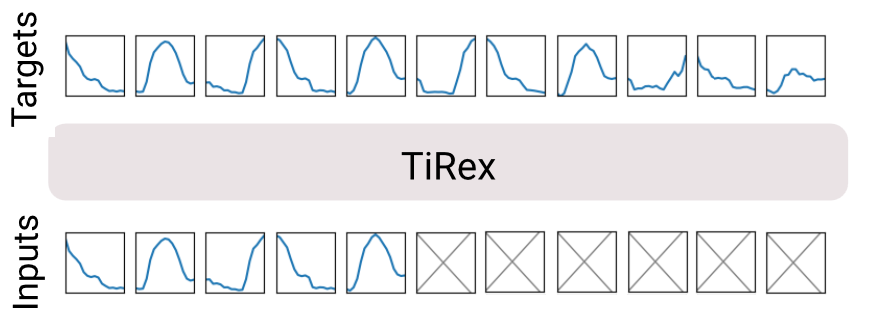
\includegraphics[width=0.8\linewidth]{images/shift.png}
	\caption{Illustration of shift method for dataloader strategy.}
	\label{fig:shift}
\end{figure}

\subsubsection{xLSTM vs. LSTM}
\label{sec:xlstm_vs_lstm}

An additional point of interest was the effect of replacing the xLSTM layer (\citeauthor{beck2024xlstmextendedlongshortterm}~\cite{beck2024xlstmextendedlongshortterm}) by a LSTM layer (\citeauthor{LSTM}~\cite{LSTM}). The rest of the architecture was kept the same.

\section{Results}
\label{sec:results}

\begin{table}[htbp]
	\centering
	\begin{threeparttable}
		\caption{Evaluation scores (big dataset)}
		\label{tab:scores_custom_tirex_full}
		\begin{tabular}{lllcccc}
			\toprule
			& & & \multicolumn{2}{c}{\textbf{SMAPE Score}} & \multicolumn{2}{c}{\textbf{Quantile Score}} \\
			\cmidrule(lr){4-5} \cmidrule(lr){6-7}
			\textbf{Dataloader} & \textbf{Layer} & \textbf{Loss} & \textbf{Autoregressive} & \textbf{Original} & \textbf{Autoregressive} & \textbf{Original} \\
			\midrule
			\multicolumn{7}{l}{{\small \emph{Custom TiRex model}}}\\
			cpm & lstm & l1         & 0.5610 & \cellcolor[HTML]{fdfebc}0.5496 & -  & -  \\
			cpm & lstm & mse        & \cellcolor[HTML]{fdfebc}0.5436 & 0.5610 & -  & -  \\
			cpm & lstm & quantile   & 0.6825 & \cellcolor[HTML]{fdfebc}0.6799 & 11.4729 & 12.4072 \\
			\addlinespace
			cpm & slstm & l1        & 0.5905 & \cellcolor[HTML]{fdfebc}0.5697 & -  & -  \\
			cpm & slstm & mse       & \cellcolor[HTML]{fdfebc}0.5553 & 0.5726 & -  & -  \\
			cpm & slstm & quantile  & \cellcolor[HTML]{fdfebc}0.6637 & 0.6795 & 11.5788 & 13.1078 \\
			\addlinespace
			shift & lstm & l1       & \cellcolor[HTML]{fdfebc}0.6691 & 0.7104 & - & - \\
			shift & lstm & mse      & 0.5670 & \cellcolor[HTML]{fdfebc}0.5582 & -  & -  \\
			shift & lstm & quantile & \cellcolor[HTML]{fdfebc}0.6745 & 0.6866 & 11.9533 & 12.7776 \\
			\addlinespace
			shift & slstm & l1      & \cellcolor[HTML]{fdfebc}0.6713 & 0.7691 & - & - \\
			shift & slstm & mse     & \cellcolor[HTML]{fdfebc}0.6578 & 0.7180 & - & - \\
			shift & slstm & quantile & \cellcolor[HTML]{fdfebc}0.6720 & 0.6888 & 11.8404 & 12.7920 \\
			\midrule
			\multicolumn{7}{l}{{\small \emph{Original pre-trained TiRex model}}}\\
			TiRex & slstm & quantile  & 0.0326 & \cellcolor[HTML]{006837}\color[HTML]{f1f1f1}0.0314 & 3.4218  & \cellcolor[HTML]{006837}\color[HTML]{f1f1f1} 3.3193  \\
			\bottomrule
		\end{tabular}
		\begin{tablenotes}
			\small
			\item[a] Lower scores indicate better predictive performance across both metrics.
		\end{tablenotes}	
	\end{threeparttable}
\end{table}

\begin{table}[htbp]
	\centering
	\begin{threeparttable}
		\caption{Evaluation scores (single sequence)}
		\label{tab:scores_custom_tirex_single}
		\begin{tabular}{lllcccc}
			\toprule
			& & & \multicolumn{2}{c}{\textbf{SMAPE Score}} & \multicolumn{2}{c}{\textbf{Quantile Score}} \\
			\cmidrule(lr){4-5} \cmidrule(lr){6-7}
			\textbf{Dataloader} & \textbf{Layer} & \textbf{Loss} & \textbf{Autoregressive} & \textbf{Original} & \textbf{Autoregressive} & \textbf{Original} \\
			\midrule
			\multicolumn{7}{l}{{\small \emph{Custom TiRex model}}}\\
			shift & lstm & l1       & \cellcolor[HTML]{fdfebc}0.0267 & 0.0913 & - & - \\
			shift & lstm & mse      & \cellcolor[HTML]{fdfebc}0.0255 & 0.0702 & -  & -  \\
			shift & lstm & quantile & \cellcolor[HTML]{fdfebc}0.1584 & 0.1678 & 4296.68 & 4673.42 \\
			\addlinespace
			shift & slstm & l1      & \cellcolor[HTML]{fdfebc}0.0321 & 0.0944 & - & - \\
			shift & slstm & mse     & \cellcolor[HTML]{fdfebc}0.0321 & 0.0841 & - & - \\
			shift & slstm & quantile & \cellcolor[HTML]{fdfebc}0.1610 & 0.1705 & 4317.57 & 4545.16 \\
			\midrule
			\multicolumn{7}{l}{{\small \emph{Fine-tuned pre-trained TiRex model}}}\\
			TiRex Or. & slstm & l1       & 0.0326 & 0.0314 & - & - \\
			TiRex Or. & slstm & mse      & 0.0326 & 0.0314 & -  & -  \\
			TiRex Or. & slstm & quantile & \cellcolor[HTML]{006837}\color[HTML]{f1f1f1}0.0201 & \cellcolor[HTML]{fdfebc}0.0202 & 441.61 & \cellcolor[HTML]{006837}\color[HTML]{f1f1f1}429.53 \\
			\addlinespace
			TiRex Auto. & slstm & l1      & 0.0326 & 0.0314 & - & - \\
			TiRex Auto. & slstm & mse     & 0.0326 & 0.0314 & - & - \\
			TiRex Auto. & slstm & quantile & \cellcolor[HTML]{006837}\color[HTML]{f1f1f1}0.0201 & \cellcolor[HTML]{fdfebc}0.0216 & 429.54 & 463.00 \\			
			\midrule
			\multicolumn{7}{l}{{\small \emph{Original pre-trained TiRex model}}}\\
			TiRex & slstm & quantile  & 0.0326 & \cellcolor[HTML]{fdfebc}0.0314 & 712.31  &  655.82  \\
			\bottomrule
		\end{tabular}
		\begin{tablenotes}
			\small
			\item[a] Lower scores indicate better predictive performance across both metrics.
		\end{tablenotes}	
	\end{threeparttable}
\end{table}


\subsection{Metrics}
\label{sec:metrics}

To compare the different methods and experiments, two main metrics are used. The symmetric mean absolute percentage error (sMAPE) and the quantile loss. The sMAPE uses only the 50\% (median) of the model output to score against the target values while the quantile loss uses all quantile predictions. For methods that do not have any quantile predictions, only the sMAPE is used.

\subsubsection{sMAPE}
\label{sec:smape}
As a general score the symmetric mean absolute percentage error (sMAPE) is used. The original definition from \citeauthor{armstrong1985long}~\cite{armstrong1985long} is slightly adapted and is defined as:
\begin{align}
	\text{SMAPE} &= \dfrac{2}{n} \sum_{t=1}^{n} \dfrac{|F_t - A_t|}{|A_t| + |F_t|}
	\label{eq:smape}
\end{align}
where $t$ is the timestep, $A_t$ the actual values and $F_t$ the forecasted values, which in our case is either the model prediction for a single output value or the median for quantile predictions. The advantage of the symmetric version is that it avoids exploding values when the actuals are close to zero and over and under-forecasts are treated in a relative way. 

\subsubsection{Quantile Loss}
\label{sec:quantile_loss}
In addition to sMAPE, the quantile (pinball) loss is used to get a measure of the individual quantile predictions. For a given quantile level $\tau \in (0,1)$, the quantile loss for a single observation $y$ and its corresponding predicted quantile $\hat{y}_\tau$ is defined as:
\begin{align}
	QL_\tau(y, \hat{y}_\tau) = \max\big(\tau \cdot (y - \hat{y}_\tau),\ (\tau - 1) \cdot (y - \hat{y}_\tau)\big)
	\label{eq:quantile_loss}
\end{align}
The overall quantile loss is obtained by averaging $QL_\tau$ over all evaluated quantile levels $\tau \in \{\tau_1, \dots, \tau_K\}$ and over all time steps $t$.


\subsection{Autoregressive}
\label{sec:autoregressive_results}

\subsection{CPM}
\label{sec:cpm_results}

\subsection{xLSTM vs. LSTM}
\label{sec:xlstm_vs_lstm_results}

\subsection{Best vs. Last Test Loss}
\label{sec:best_vs_last_results}

\begin{table}[htbp]
	\centering
	\begin{threeparttable}
		\caption{Evaluation scores (big dataset), Best vs. Last Test Loss}
		\label{tab:scores_custom_tirex_best_last}
		\begin{tabular}{lllcccc}
			\toprule
			& & & \multicolumn{2}{c}{\textbf{SMAPE Score}} & \multicolumn{2}{c}{\textbf{Quantile Score}} \\
			\cmidrule(lr){4-5} \cmidrule(lr){6-7}
			\textbf{Dataloader} & \textbf{Layer} & \textbf{Loss} & \textbf{Best} & \textbf{Last} & \textbf{Best} & \textbf{Last} \\
			\midrule
			\multicolumn{7}{l}{{\small \emph{Custom TiRex model}}}\\
			cpm & lstm & l1         & \cellcolor[HTML]{fdfebc}0.5496 & 0.5682 & -  & -  \\
			cpm & lstm & mse        & \cellcolor[HTML]{fdfebc}0.5610 & 0.5844 & -  & -  \\
			cpm & lstm & quantile   & 0.6799 & \cellcolor[HTML]{fdfebc}0.6644 & 12.4072 & \cellcolor[HTML]{fdfebc}11.9756 \\
			\addlinespace
			cpm & slstm & l1        & \cellcolor[HTML]{fdfebc}0.5697 & 0.6015 & -  & -  \\
			cpm & slstm & mse       & \cellcolor[HTML]{fdfebc}0.5726 & 0.6037 & -  & -  \\
			cpm & slstm & quantile  & \cellcolor[HTML]{fdfebc}0.6795 & 0.6867 & 13.1078 & \cellcolor[HTML]{fdfebc}12.3918 \\
			\addlinespace
			shift & lstm & l1       & \cellcolor[HTML]{fdfebc}0.7104 & 0.7106 & - & - \\
			shift & lstm & mse      & \cellcolor[HTML]{fdfebc}0.5582 & 0.5791 & -  & -  \\
			shift & lstm & quantile & 0.6866 & \cellcolor[HTML]{fdfebc}0.6658 & \cellcolor[HTML]{fdfebc}12.7776 & 13.0410 \\
			\addlinespace
			shift & slstm & l1      & \cellcolor[HTML]{fdfebc}0.7691 & 0.7797 & - & - \\
			shift & slstm & mse     & \cellcolor[HTML]{fdfebc}0.7180 & 0.7263 & - & - \\
			shift & slstm & quantile & 0.6888 & \cellcolor[HTML]{fdfebc}0.6806 & 12.7920 & \cellcolor[HTML]{fdfebc}12.4812 \\
			\bottomrule
		\end{tabular}
		\begin{tablenotes}
			\small
			\item[a] Lower scores indicate better predictive performance across both metrics.
			\item[b] Only scores from original multi-patch prediction behavior are shown.
		\end{tablenotes}	
	\end{threeparttable}
\end{table}


\section{Conclusion}
\label{sec:conclusion}

Space for your summary, central conclusions, and an outlook on potential future work.



%% 
%%%%%%%%%%%%%%%%%%%%%%%%%%%%%%%%%%%%%%%%%%%%%%%%%%%%%%%%%%%%%%%%%%%%%%%%%%%%%%%%

%%%%%%%%%%%%%%%%%%%%%%%%%%%%%%%%%%%%%%%%%%%%%%%%%%%%%%%%%%%%%%%%%%%%%%%%%%%%%%%%
%% 
%% Print the bibliography
%% 
%% (Optionally) let the bibliography start on a new odd page (odd is only relevant in twoside layout)
%\cleardoubleoddpage
\printbibliography
%% 
%%%%%%%%%%%%%%%%%%%%%%%%%%%%%%%%%%%%%%%%%%%%%%%%%%%%%%%%%%%%%%%%%%%%%%%%%%%%%%%%

%% Begin with the appendix part (all further sections will be appendices)
\appendix

%%%%%%%%%%%%%%%%%%%%%%%%%%%%%%%%%%%%%%%%%%%%%%%%%%%%%%%%%%%%%%%%%%%%%%%%%%%%%%%%
%% 
%% Add your appendix sections ...
%% 

%% Make sure to start the appendix on a new odd page (odd is only relevant in twoside layout)
%\cleardoubleoddpage
\section{An Appendix}
\label{app:an-appendix}

\subsection{Train and Test Losses, Fine-tuning pre-trained model on single sequence}
\label{sec:losses_tirex_single}

Train and test losses are visible in \autoref{tab:losses_tirex_single} and \autoref{fig:losses_tirex_single}.

\begin{table}[htbp]
	\centering
	\caption{Train Losses - Pre-trained TiRex (single sequence)}
	\label{tab:losses_tirex_single}
	\begin{tabular}{lllrrr}
		\toprule
		\textbf{Dataloader} & \textbf{Layer} & \textbf{Loss} & \textbf{Total Epochs} & \textbf{Best Train Loss} & \textbf{Best Test Loss}\\
		\midrule
		TiRex Original & slstm & quantile & 15 & \cellcolor[HTML]{006837}\color[HTML]{f1f1f1}197.24 & \cellcolor[HTML]{006837}\color[HTML]{f1f1f1}456.92 \\
		TiRex Autoregressive & slstm  & quantile & 15 & 223.38 & 457.49 \\
		\midrule
		TiRex Original & slstm & mse      & 15 & \cellcolor[HTML]{006837}\color[HTML]{f1f1f1}5,648,324.81 & \cellcolor[HTML]{006837}\color[HTML]{f1f1f1} 7,234,065.25 \\
		TiRex Autoregressive & slstm  & mse      & 15 & 6,136,206.37 & 7,673,015.60  \\
		\midrule
		TiRex Original & slstm & l1       & 15 & \cellcolor[HTML]{006837}\color[HTML]{f1f1f1}1584.60 & \cellcolor[HTML]{006837}\color[HTML]{f1f1f1}1,793.49  \\
		TiRex Autoregressive & slstm  & l1       & 15 & 1,629.62 & 1,846.40  \\
		\bottomrule
	\end{tabular}
\end{table}


\begin{figure}[htbp]
	\centering
	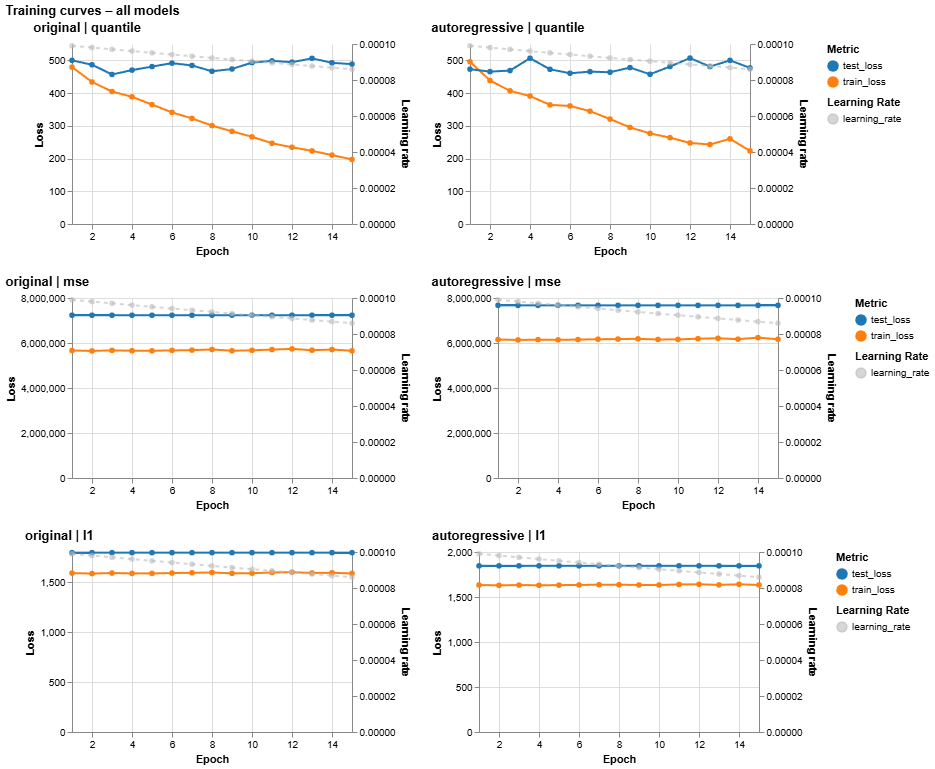
\includegraphics[width=1.1\linewidth]{images/loss_pretrain_single.png}
	\caption{Train Losses - Pre-trained TiRex (single sequence)}
	\label{fig:losses_tirex_single}
\end{figure}

\subsection{Train and Test Losses, Custom TiRex on big dataset}
\label{sec:losses_custom_tirex_full}

Train and test losses are visible in \autoref{tab:losses_custom_tirex_full} and \autoref{fig:losses_custom_tirex_full}.

\begin{table}[htbp]
	\centering
	\caption{Train Losses - Custom TiRex (big dataset)}
	\label{tab:losses_custom_tirex_full}
	\begin{tabular}{llllrrr}
		\toprule
		\textbf{Dataloader} & \textbf{Layer} & \textbf{Loss} & \textbf{Total Epochs} & \textbf{Best Train Loss} & \textbf{Best Test Loss}\\
		\midrule
		shift & slstm & quantile & 100 & 74.78 & 559.20 \\
		shift & lstm  & quantile & 100 & 41.41 & 571.46 \\
		cpm & slstm    & quantile & 100 & 42.21 & \cellcolor[HTML]{006837}\color[HTML]{f1f1f1}308.27 \\
		cpm & lstm     & quantile & 100 & \cellcolor[HTML]{006837}\color[HTML]{f1f1f1}29.07 & 322.94 \\
		\midrule
		shift & slstm & mse      & 100 & 2,901,915.03 & 4,634,443.72 \\
		shift & lstm  & mse      & 100 & \cellcolor[HTML]{006837}\color[HTML]{f1f1f1}46,591.36 & 9,396,074.49  \\
		cpm & slstm    & mse      & 100 & 97,453.89 & 8,169,185.35  \\
		cpm & lstm      & mse      & 100 & 59,365.80 & \cellcolor[HTML]{006837}\color[HTML]{f1f1f1}7,820,493.16 \\
		\midrule
		shift & slstm & l1       & 100 & 1,246.28 & 1,534.37  \\
		shift & lstm  & l1       & 100 & 1,002.50 & 1,388.01  \\
		cpm & slstm    & l1       & 100 & 144.08 & 606.34 \\
		cpm & lstm     & l1       & 100 & \cellcolor[HTML]{006837}\color[HTML]{f1f1f1}113.85 & \cellcolor[HTML]{006837}\color[HTML]{f1f1f1}593.13 \\
		\bottomrule
	\end{tabular}
\end{table}

\begin{figure}[htbp]
	\centering
	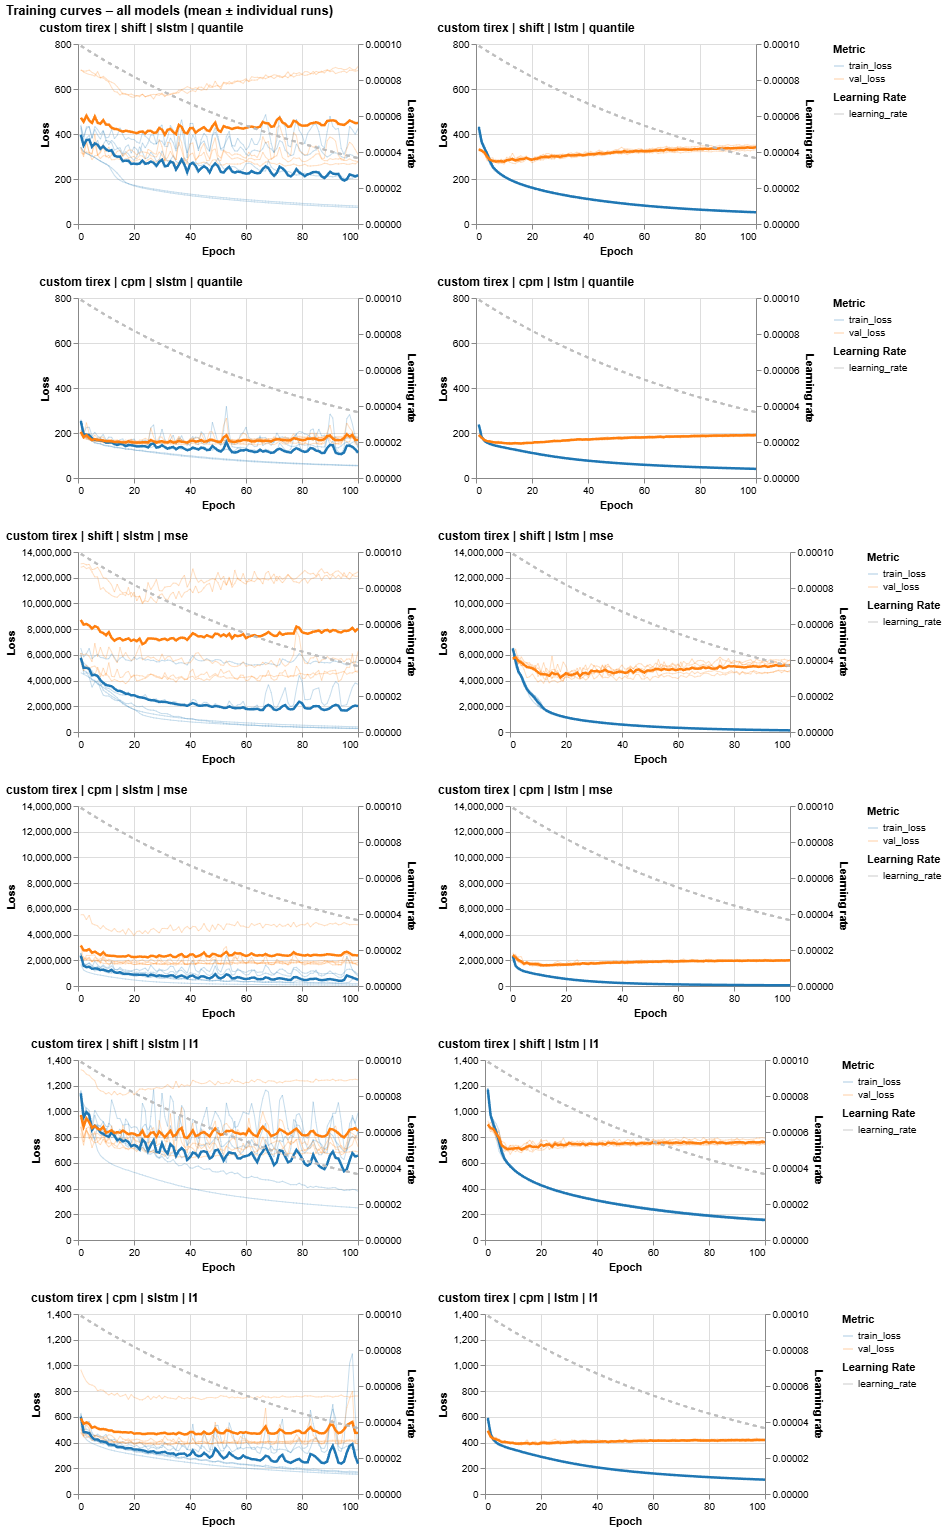
\includegraphics[width=1.1\linewidth]{images/loss_custom_full.png}
	\caption{Train Losses - Custom TiRex (big dataset)}
	\label{fig:losses_custom_tirex_full}
\end{figure}


\subsection{Train and Test Losses, Custom TiRex on single sequence}
\label{sec:losses_custom_tirex_single}

Train and test losses are visible in \autoref{tab:losses_custom_tirex_single} and \autoref{fig:losses_custom_tirex_single}.

\begin{table}[htbp]
	\centering
	\caption{Train Losses - Custom TiRex (single sequence)}
	\label{tab:losses_custom_tirex_single}
	\begin{tabular}{lllrrr}
		\toprule
		\textbf{Dataloader} & \textbf{Layer} & \textbf{Loss} & \textbf{Total Epochs} & \textbf{Best Train Loss} & \textbf{Best Test Loss}\\
		\midrule
		shift & slstm & quantile & 100 & 504.15 & 576.95 \\
		shift & lstm  & quantile & 100 & \cellcolor[HTML]{006837}\color[HTML]{f1f1f1}383.60 & \cellcolor[HTML]{006837}\color[HTML]{f1f1f1}527.99 \\
		\midrule
		shift & slstm & mse      & 100 & 3,101,287.11 & 4,775,838.26 \\
		shift & lstm  & mse      & 100 & \cellcolor[HTML]{006837}\color[HTML]{f1f1f1}1,293,486.37 & \cellcolor[HTML]{006837}\color[HTML]{f1f1f1}3,125,015.24  \\
		\midrule
		shift & slstm & l1       & 100 & 1,509.92 & 1,519.90  \\
		shift & lstm  & l1       & 100 & \cellcolor[HTML]{006837}\color[HTML]{f1f1f1}974.00 & \cellcolor[HTML]{006837}\color[HTML]{f1f1f1}1,384.28  \\
		\bottomrule
	\end{tabular}
\end{table}


\begin{figure}[htbp]
	\centering
	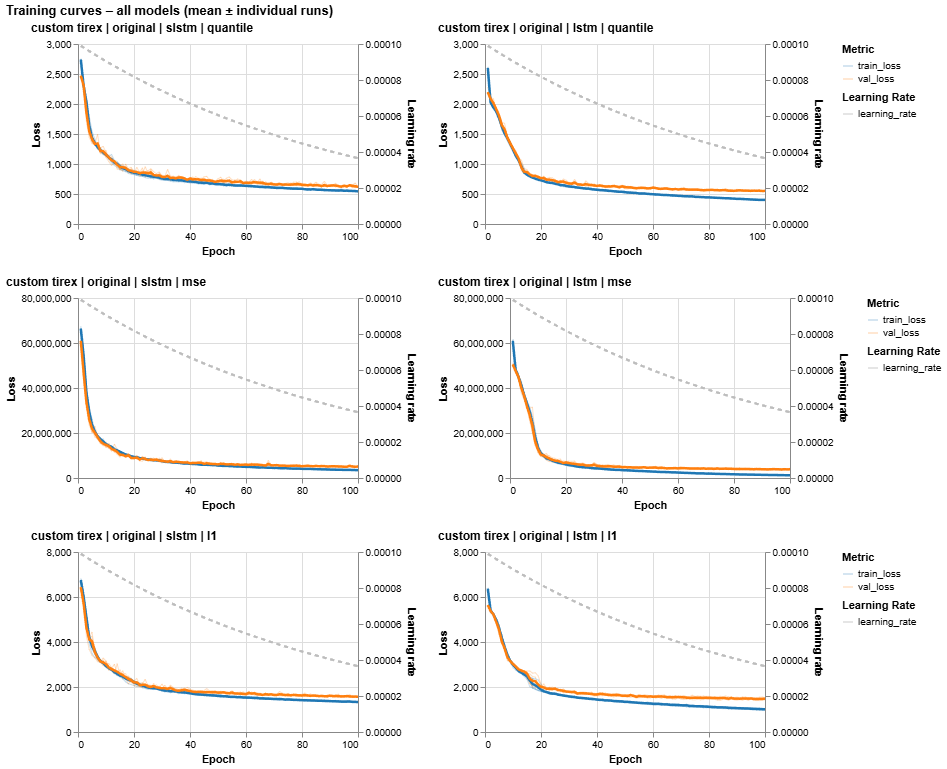
\includegraphics[width=1.1\linewidth]{images/loss_custom_single.png}
	\caption{Train Losses - Custom TiRex (single sequence)}
	\label{fig:losses_custom_tirex_single}
\end{figure}



%% 
%%%%%%%%%%%%%%%%%%%%%%%%%%%%%%%%%%%%%%%%%%%%%%%%%%%%%%%%%%%%%%%%%%%%%%%%%%%%%%%%

\cleardoubleoddpage

\end{document}
\endinput
